\chapter{The Analysis Lattice}
Inspired by TAJS we have a lattice for abstract values, $Value$, from which we build a lattice for abstract objects, $Object$. These two lattices are the main building blocks for the lattice for abstract states, $State$. Our analysis lattice is the lattice which for each program point (i.e. for each CFG node) tells the abstract state of that program point. Furthermore the analysis lattice tells the call graph of the CFG.

\subsection{Abstract Values}
The concrete lattices follows below.
\begin{eqnarray*}
Value =& Undefined \times None \times Boolean \times Integer \\
       & \times Float \times Long \times Complex \times String \times P(ObjectLabel)
\end{eqnarray*}
The value lattice is used to tell the value of a temporary variable (see the lattice Stack), and a property on an object (see the lattice Object). The $Undefined$ and $None$ lattices both contains two nodes, Top and bottom. In Python when a function does not return a value, it is the constant None\cite{pyref.constants} which is returned, e.g.:
\begin{listing}[H]
	\begin{minted}[linenos]{python}
def a(): 
	pass
a() is None // true
	\end{minted}
	\caption{Constant None}\label{code:NoneExample}
\end{listing}

\begin{wrapfigure}{r}{0.5\textwidth}
	\vspace{-20pt}
	\begin{center}
		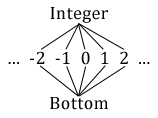
\includegraphics[width=0.48\textwidth]{images/integer-lattice.png}
	\end{center}
	\vspace{-10pt}
	\caption{The integer lattice}
	\label{fig:latticeInteger}
	\vspace{-10pt}
\end{wrapfigure}
Contrary to JavaScript, Python supports integers, floats, longs and complex numbers, so we have separate lattices for those. Note that $Complex = Float \times Float$, since a complex number in Python is represented using a float for the real and imaginary part, respectively \cite{pyref.stdtypes}. The Integer lattice is defined here in Figure \ref{fig:latticeInteger} The Float, Long and String lattices are defined in similar ways. Finally, a value can of course also be a pointer to an object in the heap, which we model in the Value lattice by having a power set\footnote{All our power sets are ordered by subset inclusion.} of object labels, $P(ObjectLabel)$.

\subsection{Abstract State}
We use the following lattice to model abstract state:
\begin{equation*}
State = Heap \times Stack
\end{equation*}
In the following sections the $Heap$ and $Stack$ lattice will be described, but first it is necessary to look at the $Object$ lattice:
\begin{equation*}
Object = (PropertyName \rightarrow Value) \times P(ObjectLabel^{*})
\end{equation*}
Having made special lattices for the 'primitive' objects there is still a need to handle the more complex objects such as function objects.
As with JavaScript you can augment objects with properties at runtime, so the lattice needs to accommodate this dynamic behavior, so
we use a map from property names to values. For some objects it is required to track the scope in which they were defined, to model the closure they are evaluated in.
Thus the object lattice is the product between ObjectValues and a scope chain modelled as a list of object labels.
\subsection{The Heap}
\begin{equation*}
Heap = (ObjectLabel \rightarrow Object)
\end{equation*}
The heap is modelled by a map from object labels to an object value. We found it benefitial to distinquise between different types of objects but still handle them in the same way in the heap.
To achieve this we made several different subclasses to the object label object, e.g. function object, which besides its name and id also holds a reference to the cfg node that is the entry node for that function.


\subsection{The Stack}
The $Stack$ lattice is defined as:
\begin{equation*}
Stack = (TempVar \rightarrow Value) \times P(ObjectLabel^{*} \times ObjectLabel)
\end{equation*}
For each temporary variable, i.e. register, we specify the value of that particular temporary variable. The power set $P(ObjectLabel^{*} \times ObjectLabel)$ specifies the scope chain ($ObjectLabel^{*}$) and variable object ($ObjectLabel$). The variable object determines which object on the heap, local variable writes should we written to. For instance we will for each program have an object on the heap, that models the module/top-level script environment \inlinecode{\_\_main\_\_}\cite{pyref.main} (this is what corresponds to the global object in JavaScript). Whenever an assignment to a variable occurs in the top-level scripting environment, e.g. \inlinecode{x=10}, the variable \inlinecode{x} is set as a property mapping to the integer 10 on the \inlinecode{\_\_main\_\_} object in the heap.
The scope chain specifies where to look in case of e.g. reading a variable that is not present on the variable object. The following simple example can be used to illustrate this:
\begin{listing}[H]
	\begin{minted}[linenos]{python}
x = 10 
def a():
	print x
	\end{minted}
\caption{Scope example}\label{code:ScopeExample}
\end{listing}
For this particular Scope example in Listing \ref{code:ScopeExample} we will have the following objects on the heap:
\begin{enumerate}
  \item The \inlinecode{\_\_main\_\_} object,
  \item The object of the function \inlinecode{a},
  \item The function object of \inlinecode{a}, and
  \item The scope object of \inlinecode{a} (which is an object similar to the \inlinecode{\_\_main\_\_} object, i.e. an object where local variables are written onto).
\end{enumerate}
In line 3 the variable object will be set to the scope object of the function a (or more precise, its label), and the scope chain will be the list containing the \inlinecode{\_\_main\_\_} object. When the variable x is read, x is not found on the variable object, so it is looked up in the scope chain, where it is found on the \inlinecode{\_\_main\_\_} object. When there are more than one object on the scope chain, those objects are of course just traversed starting from the head of the list.
In this section we try to motivate why we have three objects on the heap for each function. The object of the function a in Listing \ref{code:FunctionPropertyExample} is necessary as functions are themselves objects, as in JavaScript. For instance we can set a property on a function object as line 3 in the following example illustrates:
\begin{listing}[H]
	\begin{minted}[linenos]{python}
def a():
	pass
a.prop = 42
	\end{minted}
\caption{Property on function object}\label{code:FunctionPropertyExample}
\end{listing}
Thus we map the property prop to the integer 42 on the object of the function. Furthermore we map the magic property \inlinecode{\_\_call\_\_} to the function object of a. Whenever a function is declared in Python, the object of the function will have this property as this example illustrates:
\begin{listing}[H]
	\begin{minted}[linenos]{python}
def a():
	print "a"
a() // "a"
a.__call__ # <method-wrapper '__call__' of function object at ...> 
a.__call__() # "a"
	\end{minted}
\caption{Function object and \_\_call\_\_ example}\label{code:printFunctionExample}
\end{listing}
Thus the function object in Listing \ref{code:printFunctionExample} can be considered as the object of the method-wrapper. It is important to distinguish between the object of the function, and the function object, since \inlinecode{\_\_call\_\_} is not just a reference to the object of the function, as illustrated below:
\begin{listing}[H]
	\begin{minted}[linenos]{python}
def a(): 
	pass
a.__call__.prop = 10 # TypeError: 'method-wrapper' 
 # object has only read-only attributes
	\end{minted}
\caption{Function object and \_\_call\_\_ example}\label{code:callPropertyExample}
\end{listing}
Finally, the scope object of a function in Listing \ref{code:callPropertyExample} is necessary as local variables inside a function should not be set as properties on the object of the function:
\begin{listing}[H]
	\begin{minted}[linenos]{python}
def a(): 
	x = 42
a.x # AttributeError
	\end{minted}
\caption{Function object and \_\_call\_\_ example}\label{code:callPropertyExample}
\end{listing}
\begin{eqnarray*}
CallGraph =& (Node \times Node) \\
Analysis =& (Node \rightarrow State) \times CallGraph
\end{eqnarray*}



